\chapter{Bildverarbeitung und Umsetzung}
\label{cha:verarbeitungumsetzung}

\section{Kalibrierung}
\label{sec:kalibrierung}

F"ur eine Messung, bei der der Fehler minimiert werden soll, ist das Kalibrieren der Kameras unumg"anglich. Durch die Linse einer Kamera entsteht eine tonnenf"ormige Verzeichnung. Diese Fehler sind meist so klein, dass sie vom menschlichen Auge nicht erfasst werden k"onnen \cite{VZ} \cite{VZ1}. Durch die Kalibrierung der Kamera k"onnen diese kompensiert werden.\newline

\begin{figure}[H]
	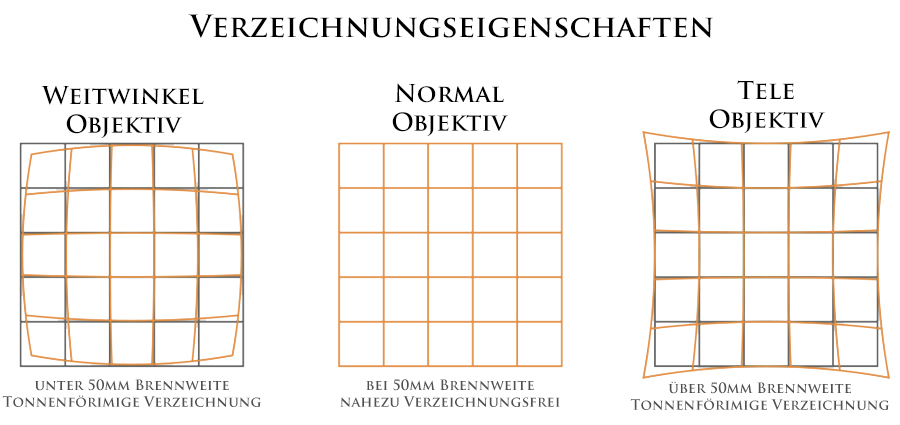
\includegraphics[scale=0.45]{bilder/verzeichnung}
	\caption[Verzeichnung]{Verzeichnung}
	\small Quelle: \url{http://www.fotokurs-bremen.de/wp-content/uploads/2016/11/Objektiv-Verzeichnung.jpg}
\end{figure}

\noindent Durch die Kamerakalibrierung werden folgende Parameter bestimmt:

\begin{description}
	\item[Intrinsische Parameter]
	Bezeichnen die Abbildung von 3D-Punkten im Kamerakoordinatensystem auf den 2D-Sensor der Kamera. Es sind Informationen der Kamera selbst, die unabh"angig davon sind, wo sich die Kamera befindet und wie diese ausgerichtet ist \cite{Intr}.
	
	\item[Extrinsische Parameter]
	Die r"aumliche Lage und Orientierung der Kamera zu einem Referenzkoordinatensystem, d.h. die Rotation und Translation \cite{cal} \cite{extr}.
\end{description}

\noindent Da es ich bei dem System um ein Stereokamera-System handelt, ist die Kalibrierung von diesem etwas komplizierter.\newline
Zuerst m"ussen die Kameras gesondert kalibriert werden. Dies wird mit der Funktion \textit{calibrateCamera} von OpenCV durchgef"uhrt. F"ur die Kalibrierung wird ein Schachbrett-Muster verwendet. Wichtig ist, dass bei der Kalibrierung beide Kameras dasselbe Bild verwenden. F"ur die Erkennung des Schachbretts wird die OpenCV-Funktion \textit{findChessboardCorners} verwendet. Diese liefert die Objekt- und Bild-Punkte der Aufnahme. Bei den Objekt-Punkten handelt es sich um die 3D-Punkte des Bildes, bei den Bild-Punkten um die 2D-Punkte \cite{OcvD}.

\begin{figure}[H]
	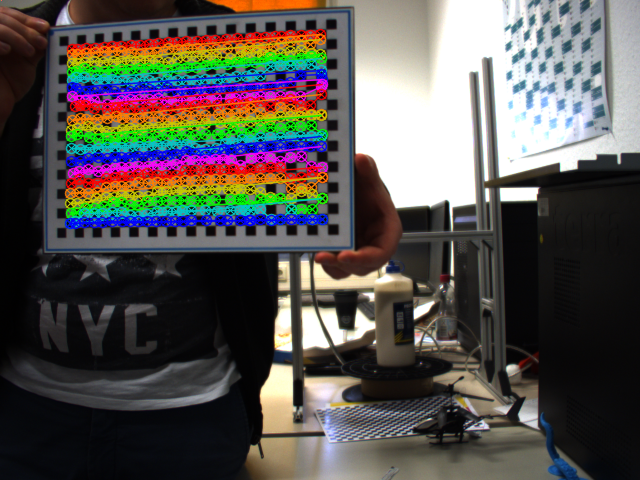
\includegraphics[scale=0.4]{bilder/calibration}
	\caption[Kalibrierung]{Kalibrierung}
\end{figure}

\noindent F"ur eine m"oglichst genaue Kalibrierung werden 50 Bilder verwendet. Anhand dieser wird jede Kamera mittels \textit{calibrateCamera} kalibriert.\newline
Die Funktion liefert die intrinsisches Parameter in Form von einer $3x3$ Kamera-Matrix

\begin{figure}[H]
	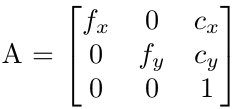
\includegraphics[scale=0.75]{bilder/matrix}
\end{figure}

\newpage

\noindent Wobei $f_{x}$ und $f_{y}$ die Brennweite in Pixeln und $c_{x}$ $c_{y}$ ein Hauptpunkt, der normalerweise in der Bildmitte liegt, ist.

\noindent Die Ergebnisse dieses Vorgangs werden auf dem Computer gespeichert, sodass dieser nicht wiederholt werden muss. Anschlie"send wird das Ergebnis der Kalibrierungen an die OpenCV-Funktion \textit{stereoCalibrate} "ubergeben.\newline
Mit Hilfe der Stereo-Kalibrierung kann der Zusammenhang zwischen den Kameras ermittelt werden: Es werden von dem Bezugsbild, welches zum Ursprung des Koordinatensystems wird, die Objekt-Punkte verwendet. Von beiden Kamerasystem werden die Bild-Punkte, die jeweiligen Kameramatrizen und die Verzeichnungskoeffizienten verwenden.

\section{Tiefeninformationen}
\label{sec:tiefeninformationen}

\noindent Das Verwenden des Stereo-Kameras ist relevant f"ur die Berechnung von Tiefeninformationen. Da die Information der Tiefe nicht in einem einzigen Bild ermittelt werden kann, wird eine zweite Kamera hinzugef"ugt. Diese ist im Raum verschoben, fotografiert aber zum gr"o"sten Teil die gleiche Szene.

\begin{figure}%
	\centering
	\subfloat[Stereosystem]{{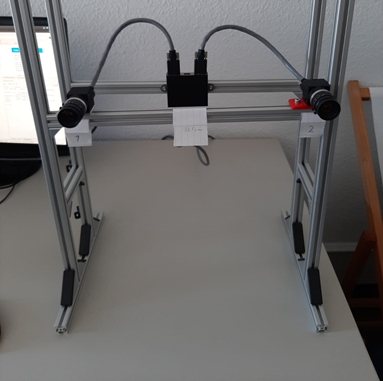
\includegraphics[width=6cm]{bilder/camerasystem} }}%
	\qquad
	\subfloat[Szenenaufnahme]{{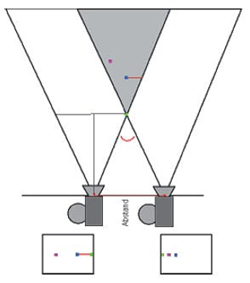
\includegraphics[width=6cm]{bilder/szene} }}%
	\caption{Stereo-System}%
	\small Quelle: \url{https://me.efi.th-nuernberg.de/interaktion/index.php5/Bearbeitung_und_Gewinnung_von_Tiefeninformation_durch_die_Kopplung_zweier_Kameras}
	\label{fig:stereo}%
\end{figure}

\noindent in \ref{fig:stereo}, im rechten Bild, ist in grau der Ausschnitt zu sehen, der von beiden Kameras erfasst wird. Das Bild daneben zeigt den Versuchsaufbau: zwei Kameras, die horizontal verschoben sind. Somit erhalten wir den Normalfall, der wie folgt beschrieben wird: \textit{Das achsparallele Stereosystem zeichnet sich durch zwei Kameras aus, die nur horizontal verschoben und deren Koordinatensysteme nicht gegeneinander verdreht sind \cite{Tu}.}\newline
\noindent Nun ist es m"oglich, "uber die Ungleichheiten des "uberlappenden Bildbereichs Tiefeninformationen zu ermitteln. Diese wird mit Hilfe der Disparit"at berechnet.\newline
Der horizontale Abstand, des gleichen Merkmals in beiden Bildern nennt man Disparit"at. \textit{Die Disparität ist umgekehrt proportional zur Tiefe. \cite{Tu}.}\newline
Durch die achsparallele Anordnung der Kameras, die nicht gegeneinander verdreht ist, kann die Z-Koordinate "uber die bekannten Kameraparameter, die Brennweite $f$ der Kameras und der Basisl"ange $B$ (Translation der Kameras zueinander), sowie die Disparit"at $D$ bestimmt werden. $D$ wird wie in \ref{fig:base} schematisch dargestellt, durch die Bildpunktverschiebung der Beiden Punkte $x$ un $x'$ berechnet. Der Z-Achsenwert berechnet sich mit der Formel $Z=\frac{f*B}{x-x'}$
 
 \begin{figure}[H]
 	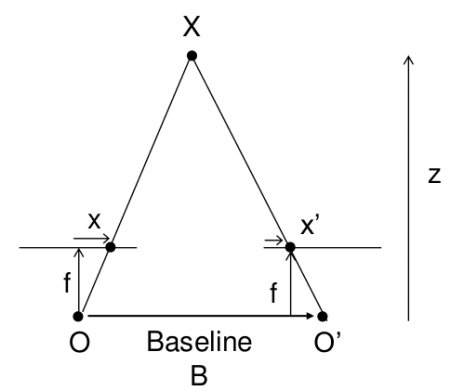
\includegraphics[scale=1.0]{bilder/tiefenberechnung}
 	\caption[Tiefenberechnung]{Tiefenberechnung}
 	\small Quelle: \url{https://opencv-python-tutroals.readthedocs.io/en/latest/py_tutorials/py_calib3d/py_depthmap/py_depthmap.html}
 	\label{fig:base}%
 \end{figure}
 
\newpage

Diese Funktion kalibriert die beiden Kameras zueinander. Dies geschieht mit Hilfe der vorher berechneten Kameramatrizen, Verzeichnungen und der Objekt- und Bild-Punkte.\newline 
Die wichtigsten Ergebnisse der Stereo-Kalibrierung sind die Rotation und die Translation der beiden Kameras zueinander.

\subsection{Fehler"uberpr"ufung}
\label{sec:fehlertest}

\section{Tiefeninformationen}
\label{sec:tiefeninformationen}

Um Tiefeninformationen aus zwei Bildern zu gewinnen, m"ussen diese zuerst rektifiziert und entzerrt werden. 
